\section*{Exercice 131 -- Cinématique -- Éolienne}
\setcounter{exo}{0}
%POLE JC

On s'intéresse à une éolienne pour particulier de puissance \SI{18}{kW} (comparée aux éoliennes
industrielles dont le diamètre du rotor peut atteindre \SI{125}{m} et qui fournissent \SI{5}{MW}).
On donne ci-dessous, la photo et la représentation sous forme de schéma cinématique de cette éolienne.


%\begin{figure}[H]
%\centering
%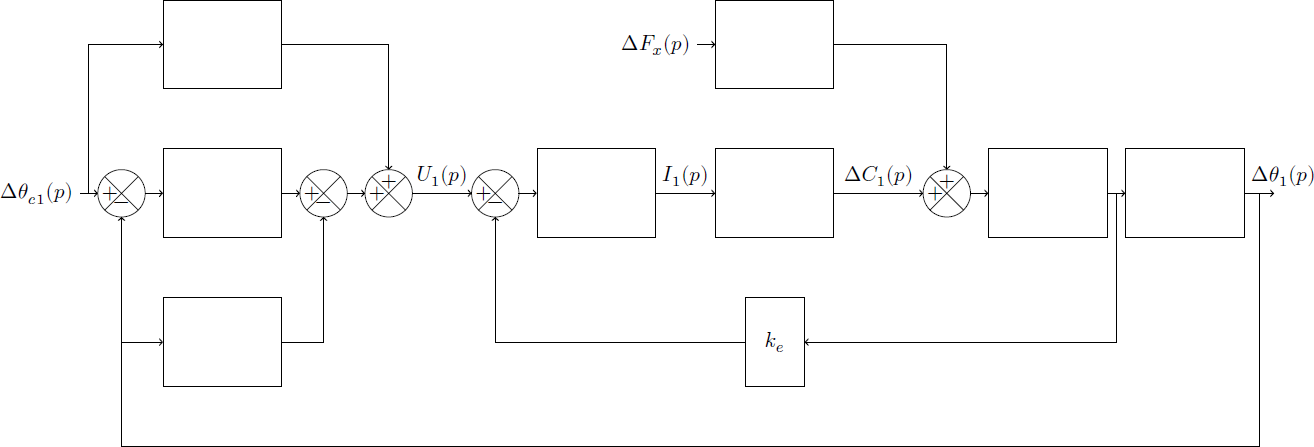
\includegraphics[width=\linewidth]{997_01}
%\end{figure}

\begin{figure}[H]
\centering
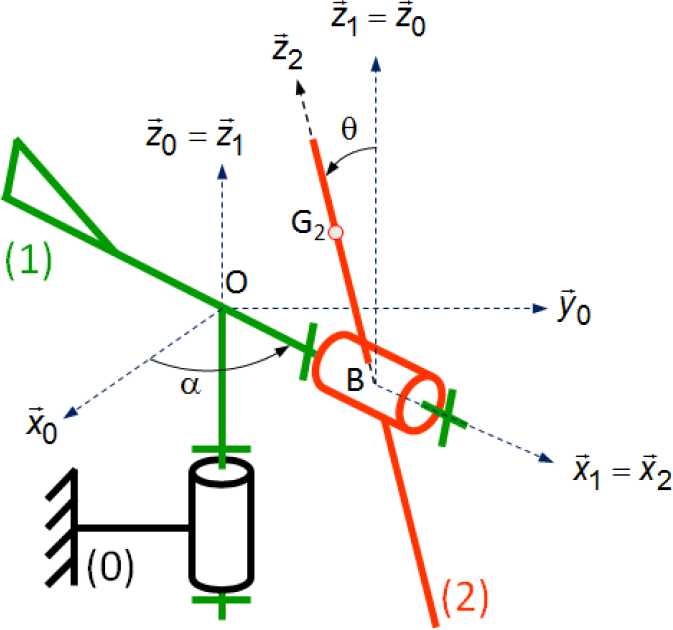
\includegraphics[width=\linewidth]{997_02}
\end{figure}

Ce système est constitué de trois solides :
\begin{itemize}
\item le mât 0, de repère associé  $\rep{0}\repere{O}{x_0}{y_0}{z_0}$, fixe par rapport au sol tel que l’axe $\axe{O}{z_0}$  soit dirigé suivant la verticale ascendante ;
\item le corps 1, de repère associé   $\rep{1}\repere{O}{x_1}{y_1}{z_1}$, en mouvement de rotation d’axe $\axe{O}{z_0}$  par rapport au mât 0 tel que $\vect{z_0}=\vect{z_1}$ et $\alpha = \angl{x_0}{x_1}$;
\item les pâles 2, de repère associé $\rep{2}\repere{B}{x_2}{y_2}{z_2}$, en mouvement de rotation d’axe $\axe{O}{z_0}$ par rapport au corps 1 tel que $\vect{OB}=b\vect{x_1}$ (b constant), $\vect{x_1}=\vect{x_2}$ et $\theta = \angl{y_1}{y_2}$.
\end{itemize}
Si un corps étranger percute une pâle au point de l'endommager, alors un « balourd » se crée (le centre de gravité $G_2$ des
pâles n’est plus sur l’axe de rotation des pâles), et des effets dynamiques (vibrations) peuvent apparaître et être à l’origine
d’effort qui vont user anormalement certaines pièces du système.
Nous poserons la position du centre de gravité $G_2$ des pâles 2 définie par $\vect{BG_2}=c\vect{z_2}$ ($c$ constant).

 \begin{obj}
Appréhender le schéma cinématique en vue d’une étude ultérieure de dynamique.
 \end{obj}



\subparagraph{}
\textit{Sur le schéma cinématique, repasser chaque solide d’une couleur différente. Repérer les liaisons et les lister
sur un graphe des liaisons. Préciser le paramètre de mouvement associé à chaque liaison.}
\ifprof
\begin{corrige}
\end{corrige}
\else
\fi


\subparagraph{}
\textit{Réaliser les figures de changement de base, et en déduire le vecteur vitesse angulaire associé à chacune
d’entre elles.}
\ifprof
\begin{corrige}
\end{corrige}
\else
\fi


\subparagraph{}
\textit{En déduire $\vecto{2}{0}$.}
\ifprof
\begin{corrige}
\end{corrige}
\else
\fi



\subparagraph{}
\textit{Décrire le mouvement de 2/1. Préciser, puis tracer sur le schéma cinématique les trajectoires $T_{G_2\in 2/1}$
$T_{B_2\in 2/1}$.}
\ifprof
\begin{corrige}
\end{corrige}
\else
\fi

\subparagraph{}
\textit{Décrire le mouvement de 1/0. Préciser, puis tracer sur le schéma cinématique les trajectoires $T_{B\in 1/0}$, 
$T_{O\in 1/0}$ et $T_{G_2\in 1/0}$.}
\ifprof
\begin{corrige}
\end{corrige}
\else
\fi